\documentclass[10pt, twocolumn, a4paper]{article}
%\usepackage{usenix,epsfig,endnotes}
\usepackage{graphicx}
\usepackage{float}
\usepackage{amsmath}
\usepackage{amssymb}
\usepackage{graphicx}
\usepackage{mathptmx}  % times roman, including math (where possible)
%\usepackage{hyperref}

\title{\Large \bf Project Plan}
\author{Jinliang Wei}
\date{\today}

\begin{document}
\maketitle
\section{Introduction}
The purpose of document is to lay out the plan of the project, its expected research contributions, and milestone to ensure progress. 

In this document, I identify some limitations of GraphChi as a disk streaming system and propose a table-based disk streaming system that overcomes GraphChi's limitations. With a few selected use cases, I plan to show that by overcoming those limitations, the proposed system can be used for a broader set of applications and can run some existing applications with better performance.

In the proposed system, data is represented as tables. User application can create multiple tables, each of which may be larger than the size of the physical machine's memory. Our system contains a \emph{table sharder} and \emph{loader}. The \emph{table sharder} partitions each table into subtables which can fit into the machine's physical memory. The \emph{loader} loads subtables from disk into memory for user program to use. Our \emph{table sharder} and \emph{loader} allows the size of each table row to change at runtime, and repartition or combine subtables to bound the size of each subtable if necessary.

Usually there are data dependencies between rows within one table or rows in different tables. Data dependency means that processing one row requires read and/or write access to another row, which might be in the same table or a different table. If we consider each table row as a vertex in graph, such dependencies can be viewed as edges in a graph. Therefore, we name such tables \emph{vertex table}. Like graph's edges which may have associated edge data, each pair of dependent rows may also have associated data. Such data can also be represented as table, which we call \emph{edge table}. For simplicity, in the rest of the proposal, the adjacent vertex rows and adjacent edge rows of a vertex is refered to as the \emph{neighborhood} of the vertex row.

For problems whose tables have fixed dependencies among rows (fixed neighborhood of each vertex row), our system provide a \emph{table partition optimizer} and a \emph{program executor}, built on top of the \emph{table sharder} and \emph{loader}. The \emph{program executor} exectues the user program on each row of all \emph{vertex tables} or a subset of them (similar to vertex program), with the vertex row's \emph{neighborhood} loaded in memory if necessary. The \emph{partition optimizer} analyzes the row dependency information given by the user, and comes up with a best-effort partition plan to minimize the amount of disk accesses needed to load in each sub-table and its neighborhood.

The rest of the document is structured as follows. In Section~\ref{sec:reviewgraphchi}, I breifly review the contributions of GraphChi and show its limitations. In Section~\ref{sec:system}, I propose the design of a new system that overcomes the limitations of GraphChi and list its expected contributions. In Section~\ref{sec:usecases}, I show the planed use cases to demonstrate the performance of the new system compared to GraphChi. Section~\ref{sec:milestones} gives the milestones.

\section{Limitations of GraphChi}
\label{sec:reviewgraphchi}
\subsection{Brief Review of GraphChi's Contributions}
GraphChi enables data mining on very large graphs with limited memory by partitioning the graph into subgraphs so that each subgraph can fit in memory. To make the subgraphs actually useful, \textbf{GraphChi's graph partitioning has the following properties}:
\begin{enumerate}
  \item \textbf{For each vertex in a subgraph, the subgraph contains all its edges (including in edges and out edges)}.
    
    This is done by partitioning the vertices into intervals so that each interval contains the same number of edges. Out edges of each vertex interval is stored on disk as one contiguous chunk, sorted by the edge's source id. Therefore, the number of disk accesses for loading each subgraph into memory is bounded by number of vertex intervals (ie. one disk read per subgraph).
 
  \item \textbf{After loading a subgraph into memory, GraphChi's execution engine executes the user program for each vertex of the subgraph. The user program may and may only access data on the corresponding vertex and the related edges.}
    
\end{enumerate}

\subsection{Limitations of GraphChi}
\label{sec:limitations}
Based on previous experiments, the following limitations of GraphChi were found:

\begin{enumerate}
  
\item \textbf{GraphChi uses coarse-grained measure for size of vertex data loaded into memory, running high risk of loading in extra vertex data and exceeds memory budget.}

GraphChi bounds the number edges in each subgraph so that the size of edge data in each subgraph does not exceed the memory budget. However, for executing each subgraph, GraphChi loads the vertices in that subgraph by iteratively loading in several vertex chunks so that the union of the chunks cover the vertices in that subgraph. Each chunk contains a fixed number of vertices (set as a constant \texttt{verticesperblock} in GraphChi code), regardless the size of the subgraph. GraphChi uses a large number for \texttt{verticesperblock} to minimize the number of disk reads, running high risk of loading in extra vertex data and. When vertex data has large size, the extra vertex data may exceed the size of memory budget and causes the user program to slow down.

For example, in the application of LDA topic modelling, with the original \texttt{verticesperblock} ($1024*1024$), due to the natrue of the application, vertex data size grows over time, the memory usage quickly exceeds the machine's physical memory size and program was slow due to large amount of page faults. The program failed after only 4 iterations due to exhausted memory. By changing the GraphChi's internal parameter \texttt{verticesperblock} to $4096$ (thanks to Aapo), the program's memory usage for procesing each subgraph was significantly reduced, program speeded up by nearly $30\%$ due to nearly no page fault.

The example shows that some applications that have large vertex data size requires precisely counting vertex data size and bounding vertex data size in each subtable. The proposed system is expected to support that feature.

\item \textbf{GraphChi does not support vertex program to access adjacent vertex data.}

In typical graph mining problems, processing a vertex usually needs access to data on that vertex's adjacent edges. GraphChi gaurantees it loads a vertex's all adjacent edges into memory before processing that vertex. There are also many problems that require access to a vertex's adjacent vertex data (examples include LDA topic modelling, ALS matrix factorization, page rank and large matrix multiplication). 

Enabling access to adjacent vertex data on GraphChi is difficult as it requires addressing two problems: 1) Although vertices are gouped according to the vertex interval that they belong to, it is difficult or impossible to group the adjacent vertices of each vertex interval together into bounded number of groupss. Therefore, loading all adjacent vertices requires potentially scan all vertex data on disk. There is a tradeoff between reducing disk seek overhead and loading unnecessary vertex data. 2) The size of adjacent vertex data of each vertex interval is hard to bound. Loading adjacent vertex data requires GraphChi's graph sharder to bound not only the vertex data and edge data in each vertex interval but also the size of adjacent vertex data.

GraphChi works around this problem via two approaches: 1) if the vertex data is not too large, store all of them in memory; 2) if the vertex data is too large to fit in memory, replicate vertex data on edges so that they can be partitioned. Clearly, the first approach cannot handle very large vertex data and the second approach has significant performance degradation, and involves complicated data synchronization problem when vertex data changes. GraphChi implements two versions of ALS matrix factorization for collaborative filtering: \emph{in-mem} with vertex data stored in memory and \emph{edge-repl} with vertex data replicated on edges. GraphChi paper shows that \emph{in-mem} takes 9.8 min and \emph{edge-repl} takes 48 min. By providing access to adjacent vertex data, our system can avoid such performance degradation when processing large amount of vertex data.

Although it is difficult to solve the first problem in general, in the new system, the \emph{partition optimizer} makes the best effort to minimize the amount of disk reads by taking advantage of the data dependency information. \textbf{Our key insight for the second problem is that even though processing a row requires the entire neighborhood of it, the processing does not need to wait until the entire neighborhood to be loaded to start. In many problems, it is possible to divide the neighborhood into subsets, preprocess each small subset without knowing the rest of them and the intermediate result is usually of small fixed size.} Let's take page rank for an example. Even though computing the rank for a page requires knowing the ranks of all pages that link to it, only the sum of those pages' ranks is really needed. Therefore, we can compute the page rank by computing partial sums. This allows processing a subtable without loading its entire neighborhood in memory.

\item \textbf{Not all problems are suitable for graph representation.}

While graph is effective for representing problems where there exist dependencies among data, not all problems can be effectively represented as graph. The major difference between graph and table-based system is that a single graph cannot effectively handle diverse vertex and edge data types but that can be easily supported with mutiple tables. Indeed, GraphChi requires all vertex data to be of the same data type, so do all the edge data. However, with diverse vertex and edge data types, many applications can be simplified or solved more efficiently. For example, in ALS matrix factorizatoin, with diverse vertex data types, the proposed system allows user vertix and movie vertex to have latent vectors of different size, potentially allowing better accuracy. Also, movie ratings can be stored on only one kind of vertices, eliminating the need for edge data.

\item \textbf{GraphChi does not repartition the graph when the size of vertex and edge data grows or shrink.}

While GraphChi allows the size of vertex and edge data change at run time, GraphChi does not repartition the graph at run time. Therefore, a subgraph may grow and exceed the memory budget. When user expects vertex and/or edge data size to grow, GraphChi suggests user set \texttt{membudget} (a configuration parameter) to a small number. This also indicates GraphChi does not gaurantee \texttt{membudget} to be a strict bound of the memory usage. 

I do not yet have use case where significant performance degradation is caused because of this limitation, so I do not yet plan to implement runtime table repartition in our new system.

\end{enumerate}
\section{System Design}
\label{sec:system}

\subsection{System Components}
\begin{figure}[h]
  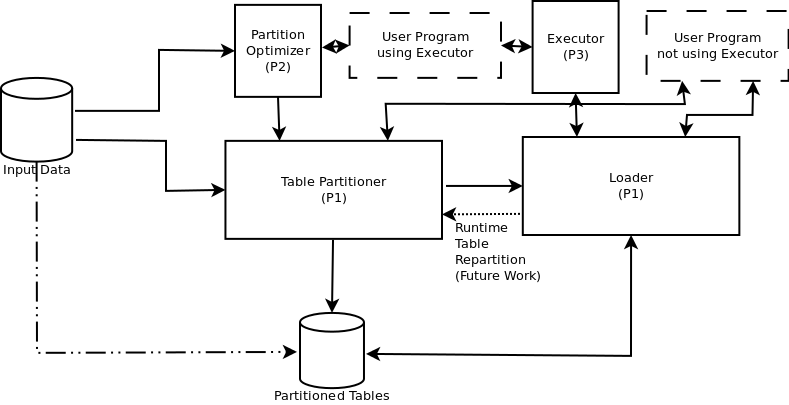
\includegraphics[width=0.5\textwidth]{graphs/system-design.png}
  \caption{System Design. Milestones are marked for each major components. P1 stands for Phase 1 and so on.}
  \label{fig:sysdesign}
\end{figure}

The system consists of the following components (as shown by the solid rectangles in Fig~\ref{fig:sysdesign}):

\begin{enumerate}
\item \textbf{Table Partitioner}. The table partitioner partitions a large amount of data into subtables and gaurantees strict bounds of each subtable's size. After partitioning, it provides user a list of handlers to subtable.
\item \textbf{Loader}. Given the subtable's id, loads the subtable into memory.
\item \textbf{Partition Optimizer} Given the data and row dependencies, comes up with a set of data partition plans. Esitmate the cost of each such plans and select the partition plan that minimizes the number of disk accesses for loading each subgraph.
\item \textbf{Executor} Execute the user program on each row of the vertex table(s), with the row's neighborhood loaded in memory.

\end{enumerate}

\subsection{Expected Contributions}

\begin{enumerate}
\item Overcomes GraphChi's limitations to gain better performance as mentioned in Section~\ref{sec:limitations}.

\item \textbf{The table partitioner and loader can be used independently.}

GraphChi only targets at single computer, so that its graph partitioner and subgraph loader are highly coupled with the program executor and does not expose interface to user. However, even in a distributed system, there are many cases where it is desirable for each individual host to handle a large amount of data which might exceeds the machine's physical memory limit. For instance, in a distributed system with dynamic scheduler, if it is equally efficient for each host to access the whole piece of data, the scheduler has much larger freedom to schedule arbitrary task on each worker node, especially in the case of straggler and node failure.

The proposed system allows the table partitioner and loader to be used independently from the rest of the system. So that user program (for example, a dynamic scheduler) may supply its own table partition plan. Moreover, this allows applications that do not execute vertex programs to use the system.
 
\end{enumerate}

\section{Use Cases}
\label{sec:usecases}
\subsection{LDA Topic Modelling}
Implemented, needs revising. Expected performance gain from proposed system.

\subsection{ALS Matrix Factorization}
Originally implemented by GraphChi, needs revising. Expected performance gain.

\subsection{Page Rank}
Originally implemented by GraphChi, needs revising. Expected to show the proposed system supports graph mining problems as GraphChi does without performance loss.

\subsection{Matrix Multiplication}
Multiplying two very large matrices, none of which fits in memory. Not yet implemented. Not supported by GraphChi.

\section{Milestones}
\label{sec:milestones}
\begin{tabular}{|l | c | r |}
\hline
Phases & Date & Milestones\\
\hline
Phase 1 & March 25 & Table Partitioner and Loader \\
\hline
Phase 2 & April 15 & Optimizer* \\
\hline
Phase 3 & April 25 & Executor \\
\hline
Phase 4 & May 5 & Examples and Evaluation \\
\hline
\end{tabular}

*Optimization plans are not yet fully decided. There are chances that the progress for optimizer is delayed.
\end{document}